\chapter[Metodologia]{Metodologia}
A metodologia escolhida para o desenvolvimento da plataforma será a metodologia ágil, a metodologia principal que vai será utilizada é o Kanban, porém, não será utilizada sua forma pura, e sim com algumas modificações, que atendem as necessidades do projeto. A escolha dessa metodologia se dá pelas seguintes características: o projeto será desenvolvido de maneira incremental, ou seja, ele poderá ser modificado no decorrer da implementação; a equipe consiste em apenas uma pessoa, o que descarta a possibilidade de utilizar o Scrum ou XP (\textit{Extreme Programming}); o escopo do projeto será divididos em tarefas, e a utilização do Kanban facilita no descobrimento de gargalos.

A metodologia Kanban surgiu no Japão com o TPS (Sistema Toyota de Produção) \cite{tps} para controlar a fabricação de automóveis e foi inserida no meio de desenvolvimento de software no ano de 2007. Kanban é um termo japonês para sinal visual e uma das grandes características dessa metodologia é evidenciar os problemas existentes no processo. 

A metodologia ágil surgiu no ano de 2001, com a reunião de especialistas em processos de desenvolvimento de software para discutir maneiras de melhorar o desempenho em projetos, com isso foi criado o Manifesto Ágil \cite{agil}. Uma das características das metodologias ágeis são sua capacidade de adaptar a novos fatores durante o desenvolvimento do projeto, ao invés de tentar prever o que pode acontecer e o que não pode
\section{Requisitos}
Os requisitos do projeto serão classificados em três níveis de hierarquia:  épicos, \textit{features} e \textit{user stories}. Os épicos são compostos por \textit{features} e representam macro entregáveis do projeto e geralmente são descritos como o nível mais abstrato. As \textit{features} são agrupamentos de \textit{user stories} e representam funcionalidades do sistema. User stories são pequenas partes de uma funcionalidade do sistema e que serão implementadas. \textit{User stories} também podem ser classificadas como \textit{technical stories} e estas \textit{technical stories} representam atividades que não agregam muito valor ao cliente, porém agregam melhoras internas no software.

No contexto do projeto as \textit{features} serão equivalentes às \textit{milestones}, e as \textit{stories} (\textit{users} ou \textit{technical}) serão as \textit{issues}. Para uma melhor visualização dos requisitos do projeto, será montado uma matriz de rastreabilidade para cada epico, sendo mostrado nas figuras \ref{image:ep01}, \ref{image:ep02} e \ref{image:ep03}.
\begin{figure}
\centering
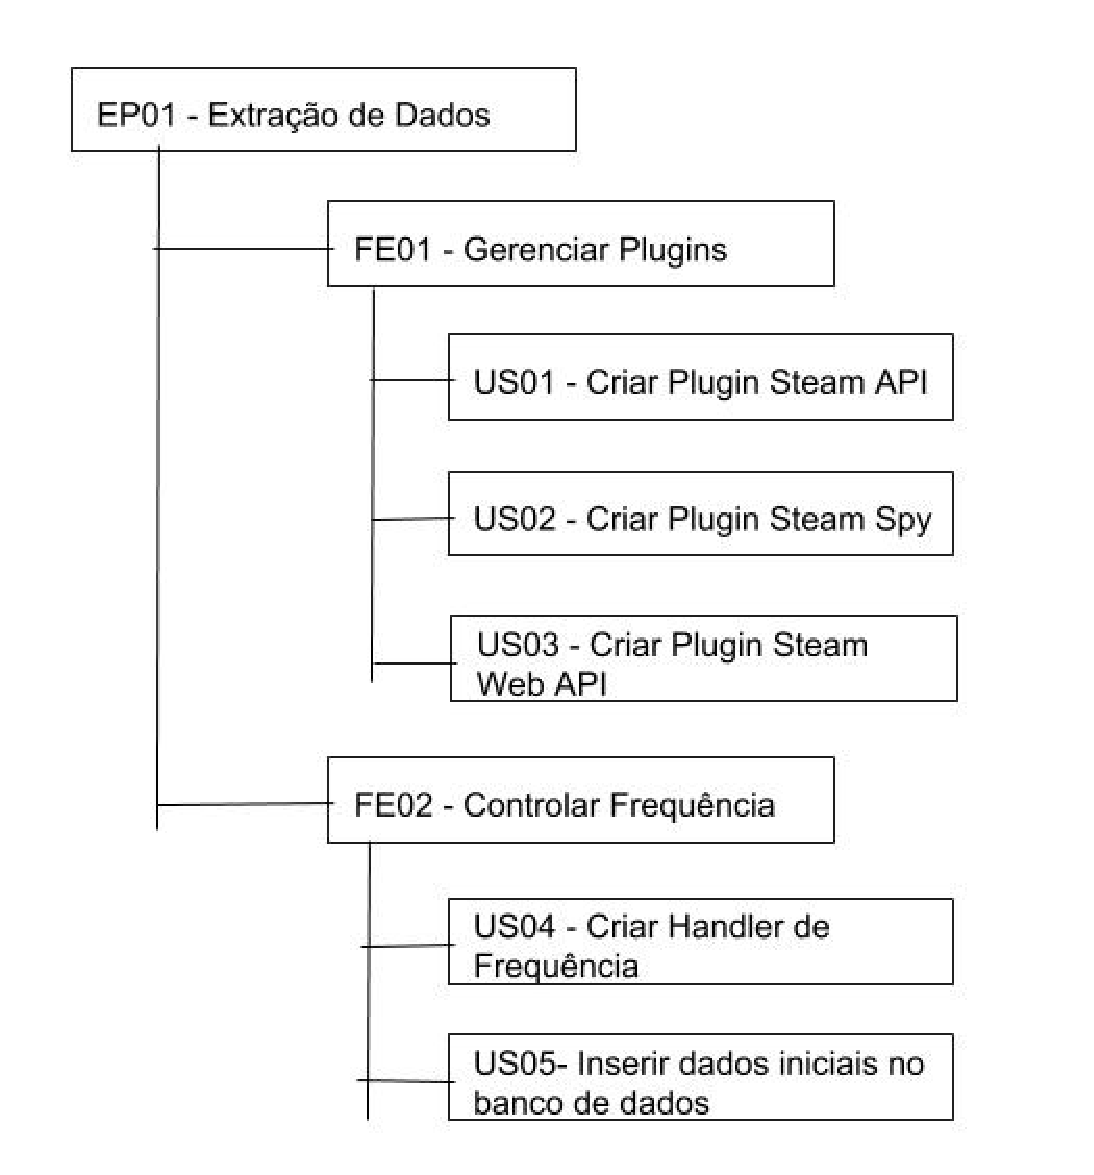
\includegraphics[scale=0.35]{figuras/EP01.eps}
\caption{Matriz Rastreabilidade Épico 1}
\label{image:ep01}
\end{figure}
\begin{figure}
\centering
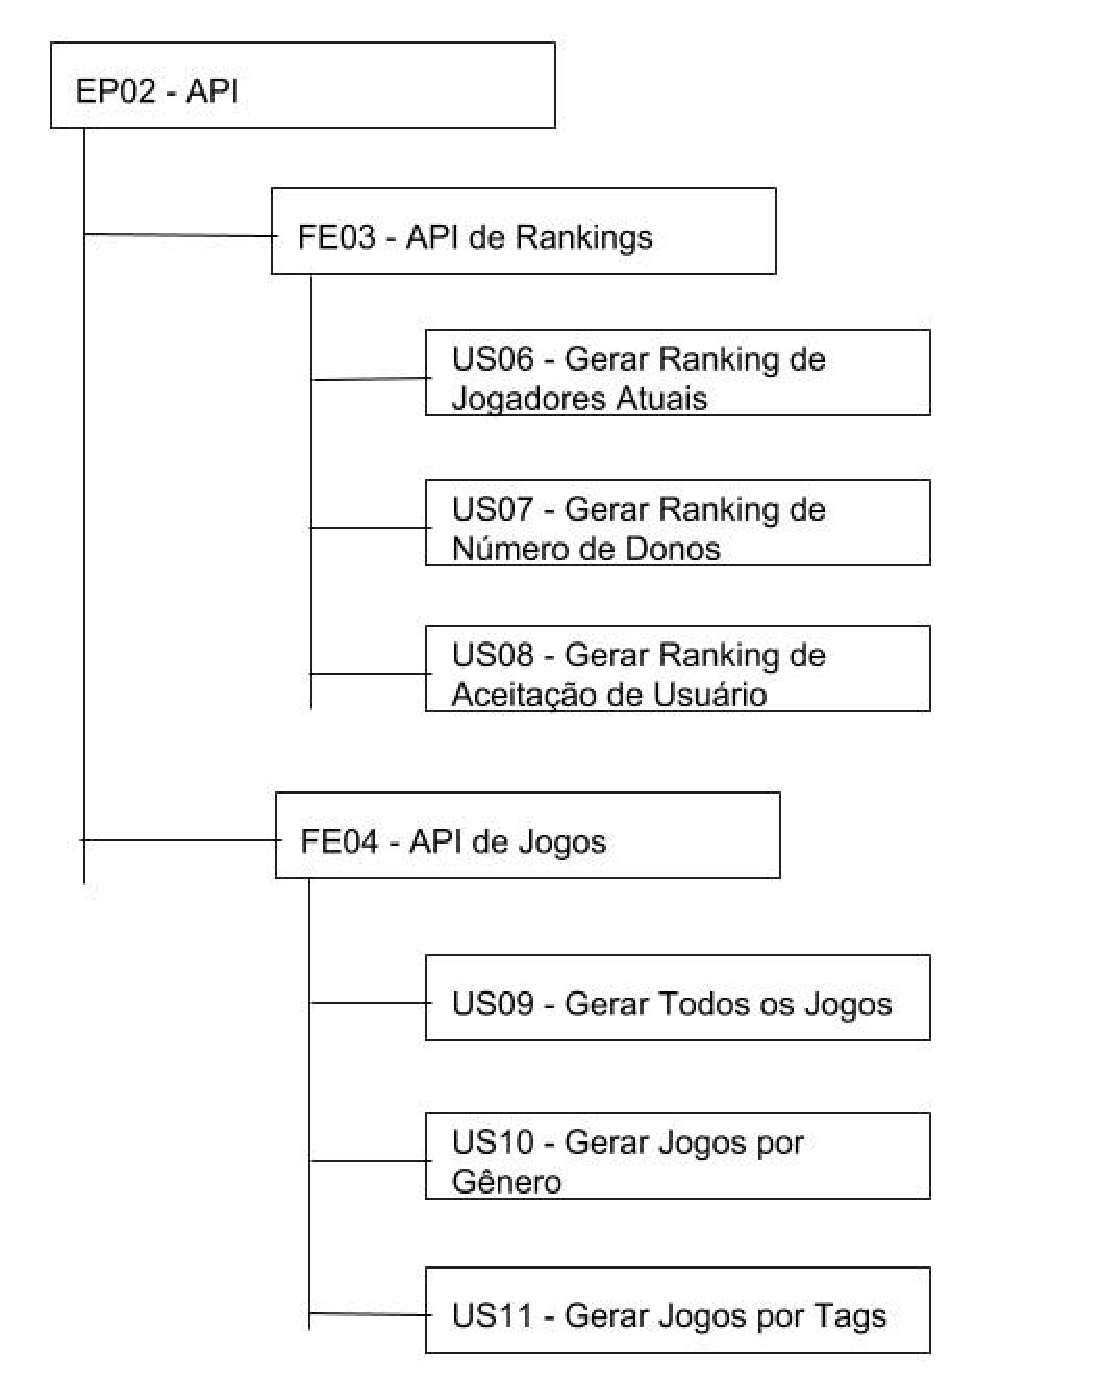
\includegraphics[scale=0.35]{figuras/EP02.eps}
\caption{Matriz Rastreabilidade Épico 2}
\label{image:ep02}
\end{figure}
\begin{figure}
\centering
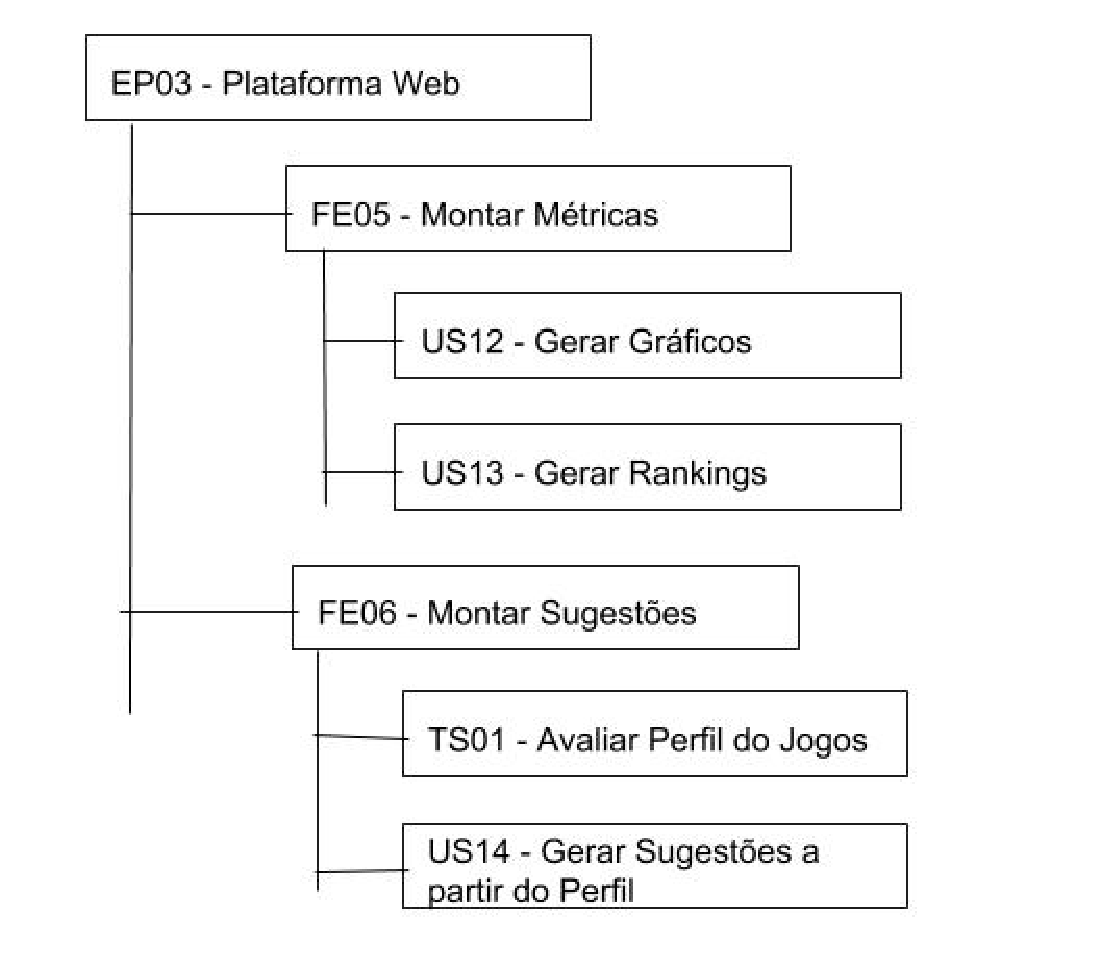
\includegraphics[scale=0.35]{figuras/EP03.eps}
\caption{Matriz Rastreabilidade Épico 3}
\label{image:ep03}
\end{figure}
\section{Análise de Ferramentas}
Nesta seção são feito estudos sobre as possíveis ferramentas que poderão ser utilizadas durante o desenvolvimento do trabalho.
\subsection{Banco de Dados}
A ferramenta de banco de dados é responsável pelo armazenamento dos dados extraídos nas fontes de dados. No contexto desse projeto, este banco deverá armazenar os dados de todos os jogos disponibilizados pela API\footnote[1]{Conjunto de rotinas e padrões de programação para acesso a um aplicativo de software ou plataforma baseado na Web} (\textit{Application Programming Interface}) da Steam.
\subsubsection*{PostgreSQL}
Postgre é uma ferramenta \textit{open source} de banco de dados que utiliza a linguagem SQL em conjunto com outras funcionalidades que guardam e manipulam os mais complicados dos dados. Postgre é uma ferramenta antiga tendo sua origem datada no ano de 1986 \cite{postgresql}.

Postgre é uma ferramenta que possui funcionalidades que auxiliam desenvolvedores e administradores a manter a integridade dos dados e criar sistemas com tolerância a falhas.
\subsubsection*{Elasticsearch}
Elasticsearch é uma ferramenta \textit{open source}, desenvolvida pela Elastic\footnote[2]{\url{https://www.elastic.co/}}, de análise e busca REST\footnote[3]{REST é uma abstração da arquitetura da Web} (\textit{Representational State Transfer}) capaz de resolver um grande número de casos. É a parte principal de Elastic Stack, servindo como um centro de armazenamento de dados \cite{elasticsearch}.

Elasticsearch suporta qualquer tipo de dado, além de agregar grande quantidades de dados para se ter uma visão melhor. Entre suas características as que mais se destacam são sua rapidez de busca, capacidade de detecção de falhas, múltiplos tipos de dados e suporte a múltiplas linguagens de programação.
\subsection{Extração de Dados}
A ferramenta de extração de dados é responsável pela extração dos dados das fontes de dados, além de ter que fazer a comunicação com o banco de dados. Essa ferramenta deverá extrair os dados das APIs que serão utilizadas, manipulá-los e inserir no banco de dados.
\subsubsection*{Logstash}
Logstash é a ferramenta de extração de dados, desenvolvida pela Elastic, ele faz parte de Elastic Stack em conjunto com o Elasticsearch. Entre as características as que mais destacam são sua capacidade de conseguir extrair qualquer tipo de dado, além de permitir a criação de filtros para transformar e manipular os dados extraídos e também permite uma gama de outputs para onde o dado será enviado \cite{logstash}.
\subsubsection*{Owner}
Outra opção de extração de dados é a criação de um software específico para a plataforma. Este software seria criado na linguagem Ruby\footnote[4]{\url{https://www.ruby-lang.org/pt/}} que também possui ligação com o Elasticsearch. As vantagens desse tipo de software seria a possível implementação de uma arquitetura de \textit{\textit{plugins}}, de modo que outros tipos de dados seriam aceitos na plataforma, além de que, caso futuramente seja necessário a mudança do banco de dados, a adaptação para o novo banco seria menos custosa.
\subsection{Frequência na Extração dos Dados}
A ferramenta da frequência de dados é mais um auxiliar na hora da extração de dados. Como serão extraídos dados que possuem uma taxa de modificação grande, é necessário utilizar uma ferramenta que crie rotinas para essa extração.
\subsubsection*{\textit{Cronjob}}
\textit{Cronjob}\footnote[5]{\url{https://cron-job.org/en/}} é uma ferramenta de agendamento que permite controlar tarefas a serem executadas em tempos pré-configurados. Através dela é possível configurar tarefas automáticas a serem executadas em um horário específico. \textit{Cronjobs} são configurados manualmente pelo terminal, podendo serem configurados para atualizações por minutos, horas, dias (do mês ou da semana) e meses
\subsubsection*{\textit{Whenever}}
\textit{Whenever} é uma \textit{gem}\footnote[6]{Gems são como bibliotecas para a linguangem Ruby} do \textit{ruby}, mais especificamente para o \textit{framework} rails. Está \textit{gem} utiliza os \textit{cronjobs} como fundo para gerenciar e controlar tarefas a serem executadas em rotinas ou em um horário específico \cite{whenever}.
\subsubsection*{\textit{Clockwork}}
\textit{Clockwork} é uma \textit{gem} do \textit{ruby}. Está \textit{gem} também utiliza os \textit{cronjobs}, porém diferente de \textit{whenever}, ele não exige que o software possua uma arquitetura MVC\footnote[7]{É um padrão de arquitetura de software} (\textit{Model-View-Controller}). Ele é utilizado especificamente para a criação de rotinas para tarefas que serão executadas automaticamente pela \textit{gem} \cite{clockwork}.
\section{Arquitetura do Projeto}
A arquitetura do projeto é dividida em cinco partes: as fontes de dados, o software de extração, o banco de indexação, a API de consumo e a plataforma web. A ligação entre as partes e sua posição na arquitetura ficam evidenciado na figura \ref{image:arquitetura}.
\begin{figure}
\centering
\includegraphics[scale=0.3]{figuras/arquiteturaGeral.eps}
\caption{Arquitura Geral do Projeto}
\label{image:arquitetura}
\end{figure}
\begin{itemize}
\item \textbf{Fonte de Dados}: é a parte onde se concentra os dados que serão utilizados para o desenvolvimento da plataforma web, estes dados poderão vir de um banco de dados, de funções \textit{crawlers}, de alguma API ou de um arquivo local.
\item \textbf{Software de Extração}: é a parte onde será feito a extração, manipulação e armazenamento dos dados que estavam nas fontes de dados. O software de extração é dividido em três componentes principais, sendo eles: o \textit{handler}, a classe \textit{main} e os \textit{plugins}. A arquitetura do software de extração e a interação entre seus componentes são demonstrados na figura \ref{image:extracao}.
\item \textbf{Banco de Indexação}: é a parte responsável por guardar os dados extraídos das fontes de dados pelo software de extração. Como a Steam possui muito jogos, o banco de indexação que será usado deverá suportar um grande número de dados e também possuir uma rapidez na hora da busca. O banco de dados escolhido foi o Elasticsearch, por que além de suportar grandes quantidades de dados e ser rápido, ele também disponibiliza certa estatísticas sobre os dados e ser suportado por muitas linguagens de programação.
\item \textbf{API de Consumo}: é a parte que permite que mais de uma plataforma possa utilizar os dados que foram guardados no banco de indexação.
\item \textbf{Plataforma Web}: é a parte onde será mostrado as métricas levantadas para o auxílios das desenvolvedoras.
\end{itemize}
\begin{figure}
\centering
\includegraphics[scale=0.35]{figuras/softwareExtracao.eps}
\caption{Arquitura do Software de Extração}
\label{image:extracao}
\end{figure}
\section{Software Extração}
O software de extração é a primeira parte propriamente dita que faz parte do projeto, nela é onde será feito a extração dos dados das fontes de dados, a manipulação necessária e a inserção dos dados no banco de indexação numa determinada frequência. Fontes de dados, como já citados na arquitetura do projeto, são os arquivos que contém os dados que serão inseridos no banco de indexação. No escopo inicial serão utilizados três fontes de dados:
\begin{itemize}
	\item \textbf{Steam Web API}: É uma API REST disponibilizada pela Steamworks\footnote[8]{\url{https://partner.steamgames.com/}}, ou seja, é uma API oficial da Steam \cite{steam_api}. Ela possui tanto métodos públicos, tanto métodos privados. Os métodos públicos são abertos para qualquer pessoas visualizar, já os métodos privados é necessário uma chave de desenvolvedor cedido pela própria Steamworks. Para acessar seus dados é preciso, além da chave, a interface na qual aquele dados está guardado, o id do jogo, caso a informação seja de um jogo, ou do id do usuário, caso a informação seja de algum usuário.
	\item \textbf{Steam Store API}: É uma API REST disponibilizada pela Steam, que não possui uma página oficial para ela. Ela disponibiliza os dados dos jogos que estão guardados no banco de dados da Steam. Para acessar seus dados e preciso saber apenas o id do jogo, porém é possível passar filtros também.
	\item \textbf{Steam Spy API}: É uma API REST disponibilizada pelo Steam Spy \cite{steam_spy}, ela é muito parecido com a Steam Store API, porém ela disponibilizada dados que apenas o Steam Spy possui, como o número de donos de um jogo ou o número de avaliações positivas e negativas de um jogo. Para acessar seus dados é preciso saber apenas o id do jogo, porém também é possível passar filtros.
\end{itemize}
Com os \textit{logs} definidos, é preciso saber quais dados das fontes de dados serão inseridos no banco de indexação, pois muitas APIs possuem dados repetidos e nem todo os dados são interessante para se manter. Com isso os principais dados que serão mantidos no banco de indexação são:
\begin{itemize}
	\item \textbf{Nome}: É o nome do jogo em questão, este dado é guardado apenas para uma referenciação, pois ele não será utilizado na montagem das métricas.
	\item \textbf{Steam Id}: É o id do jogo, esse número é necessário pois é a partir dele que serão extraídas as informações das APIs.
	\item \textbf{Descrição}: É uma breve descrição sobre o jogo, este dado será guardado apenas para uma referenciação, pois ele não será utilizado na montagem das métricas.
	\item \textbf{Desenvolvedora}: É o nome da empresa que desenvolveu o jogo, este dado será guardado, pois será levantado o número de desenvolvedoras que são a própria publicadora.
	\item \textbf{Publicadora}: É o nome da empresa que publicou aquele jogo, este dado será guardado, pois será levantado o número de desenvolvedoras que são a própria publicadora.
	\item \textbf{Preço}: É o preço em reais daquele jogo, este dado será guardado, pois será levantando o preço médio que um jogo em determinado perfil geralmente têm.
	\item \textbf{Categorias}: São as categorias que aquele jogo abrange, geralmente são mostradas como características que aquele jogo têm, este dado será guardado, pois a partir de determinadas categorias que um determinado perfil de jogos, poderá levantar sugestões para a melhoria daquele perfil.
	\item \textbf{Gêneros}: São os gêneros daquele jogo, este dado será guardado, pois a partir de um determinado gêneros, novas métricas serão montadas.
	\item \textbf{Data de Lançamento}: É a data de lançamento daquele jogo, este dado será guardado, pois com ele será montado uma métrica de quais mês um jogo com um determinado perfil foi mais lançado.
	\item \textbf{Linguagens Suportadas}: São as línguas que aquele jogo suporta, este dado será guardados, pois será levantado quais linguagens um jogo com determinado perfil possui mais suporte.
	\item \textbf{Número de Donos}: É o número médio de donos que aquele jogo têm, este dado será guardado, pois será levantada uma média de númerod de donos que um determinado perfil atingiu.
	\item \textbf{Avaliações Positivas e Negativas}: São o número de avaliações positivas e negativas que um jogo têm, este dado será guardado pois com ele será possível determinar a porcentagem de avaliações positivas que um jogo teve, e com isso será levantado uma média desta porcentagem que um determinado perfil atingiu.
	\item \textbf{Número de Jogadores Atuais}: É o número de jogadores que estão jogando um determinado jogo naquele momento, este dado será guardado, pois com ele será possível gerar \textit{rankings} de quais jogo de um determinado perfil estão sendo mais jogados.
\end{itemize}
Com os dados definidos, é preciso definir como será feito o software de extração. O software de extração será feito utilizando a linguagem de programação Ruby, com integração com o Elasticsearch. Para a atualização frequente dos dados será utilizado a \textit{gem} \textit{Clockwork}.
\section{API de Consumo}
A API de consumo será responsável por consumir o banco de indexação, e partir dos dados gerar \textit{end points} REST para que qualquer aplicação possa utilizá-la. A API deverá atualizar seus \textit{end points} com a mesma frequência com o qual o software de extração atualiza o banco de indexação.

A API possuirá dois \textit{end points}: uma para gerar informações sobres os jogos no banco de indexação e outro para gerar \textit{rankings} para um determinado perfil.

O \textit{end point} de informações dos jogos poderá receber vários filtros, sendo os mais comuns: pegar todos os jogos disponíveis no banco de indexação, pegar todos os jogos de um ou mais gêneros, pegar todos os jogos com uma ou mais determinadas categorias. Os \textit{end points} mais comuns são:
\begin{itemize}
	\item \textit{https://api/games/all}
	\item \textit{https://api/games/genre=action}
	\item \textit{https://api/games/categories=atmospheric}
\end{itemize}
O \textit{end points} de \textit{rankings} gerarão \textit{rankings} a partir de determinados filtros, sendo os mais comuns: gerar um \textit{rankings} pelos jogos mais jogados naquele momento, gerar um \textit{rankings} com os jogos que possui as maiores porcentagens de avaliações positivas. A API também deverá gerar qualquer ranking com os filtros de gêneros e categorias, ou seja, deve-se gerar um ranking qualquer para um determinado perfil de jogo. Os \textit{end points} mais comuns são:
\begin{itemize}
	\item \textit{https://api/rankings/all}
	\item \textit{https://api/rankings/current}
	\item \textit{https://api/rankings/avaliation}
\end{itemize}
\section{Plataforma Web}
A Plataforma Web é a parte principal do projeto, nela é onde será mostrado as métricas que serão montadas a partir dos dados extraídos dos \textit{logs}. A plataforma será desenvolvida em algum \textit{framework} de JavaScript, retirando os dados da API de consumo.

Outra funcionalidade importante para a plataforma web é a habilidade de fazer sugestões a partir de um determinado perfil de jogo. As sugestões serão a adição ou remoção de um gênero ou categoria no perfil, para que este tenha uma aumento no seus número de vendas ou no número da porcentagem de avaliações positivas.

As métricas que serão disponibilizadas inicialmente pela plataforma são:
\begin{itemize}
	\item Número total de jogos que atendam aquele determinado perfil. A figura \ref{image:num_total} é uma representação da métrica.
	\begin{figure}
	\centering
	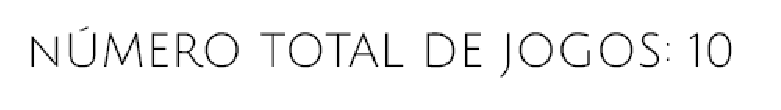
\includegraphics[scale=0.5]{figuras/num_jogos.eps}
	\caption{Número total de jogos}
	\label{image:num_total}
	\end{figure}
	\item Número médio de donos que um jogo que atende aquele determinado perfil. A figura \ref{image:med_donos} é uma representação da métrica.
	\begin{figure}
	\centering
	
\includegraphics[scale=0.5]{figuras/media_donos.eps}
	\caption{Número médio de donos}
	\label{image:med_donos}
	\end{figure}
	\item Média das porcentagens de avaliações positivas de um jogo que atende aquele determinado perfil. A figura \ref{image:avaliacoes} é uma representação da métrica.
	\begin{figure}
	\centering
	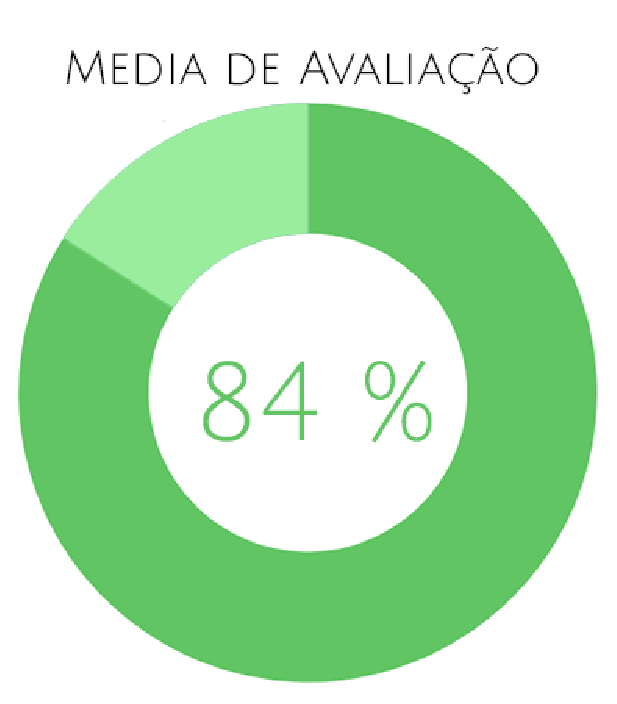
\includegraphics[scale=0.3]{figuras/avaliacao.eps}
	\caption{Média das porcentagens de avaliações positivas}
	\label{image:avaliacoes}
	\end{figure}
	\item Mês que possui o maior número de lançamento que atendam aquele determinado perfil. A figura \ref{image:mes} é uma representação da métrica.
	\begin{figure}
	\centering
	
\includegraphics[scale=0.5]{figuras/mes.eps}
	\caption{Mês com mais lançamentos}
	\label{image:mes}
	\end{figure}
	\item Gráfico de lançamentos por mês que atendam aquele determinado perfil. A figura \ref{image:lancxmes} é uma representação da métrica.
	\begin{figure}
	\centering
	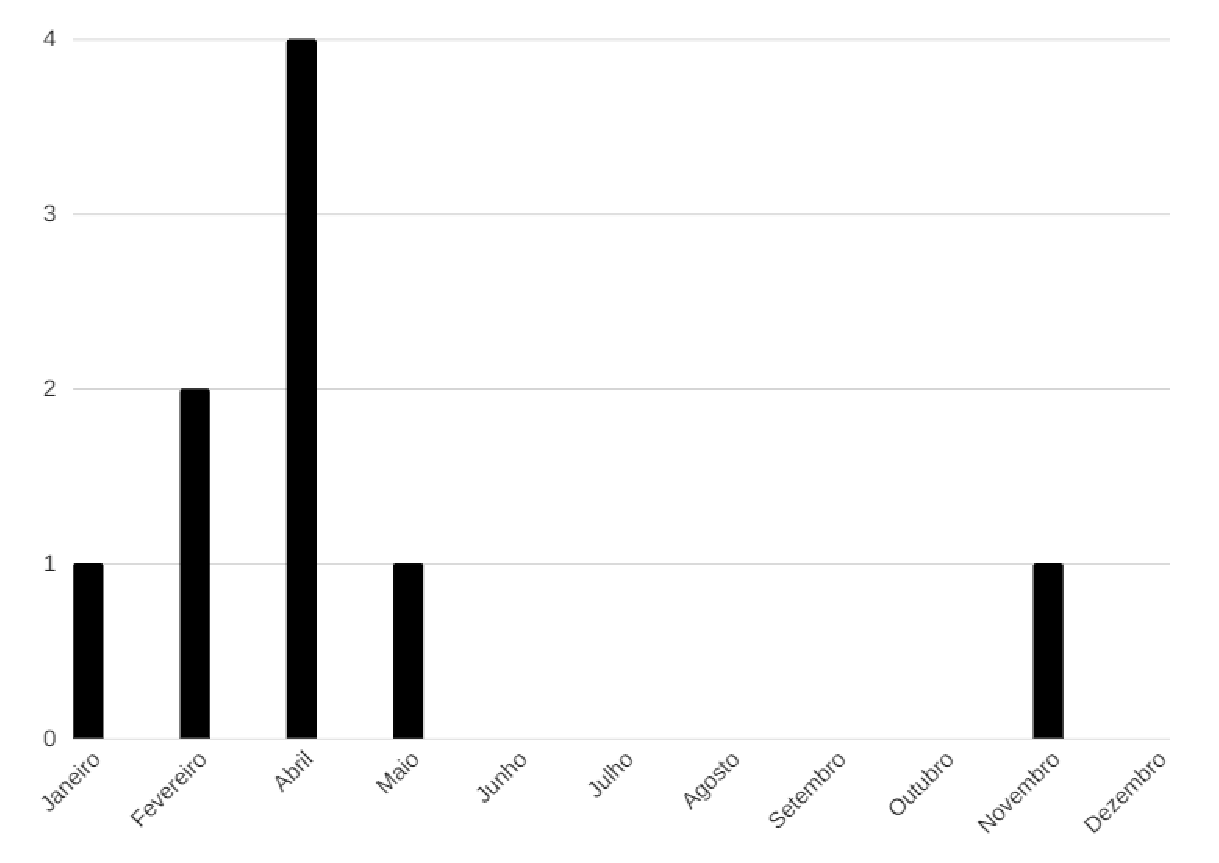
\includegraphics[scale=0.4]{figuras/lancamentoxmes.eps}
	\caption{Lançamentos x Mês}
	\label{image:lancxmes}
	\end{figure}
	\item Preço médio de um jogo que atende aquele determinado perfil. A figura \ref{image:preco} é uma representação da métrica.
	\begin{figure}
	\centering
	
\includegraphics[scale=0.5]{figuras/preco_medio.eps}
	\caption{Média dos preços}
	\label{image:preco}
	\end{figure}
	\item Número de jogos que foram publicados pela própria desenvolvedora que atendam aquele determinado perfil. A figura \ref{image:own} é uma representação da métrica.
	\begin{figure}
	\centering
	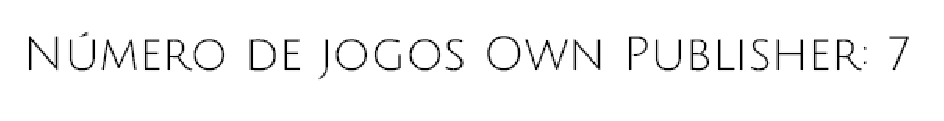
\includegraphics[scale=0.5]{figuras/own_publisher.eps}
	\caption{Número de jogos publicados pela propria desenvolvedora}
	\label{image:own}
	\end{figure}
	\item Número de jogos que foram publicado por outra empresa que atendam aquele determinado perfil. A figura \ref{image:another} é uma representação da métrica.
	\begin{figure}
	\centering
	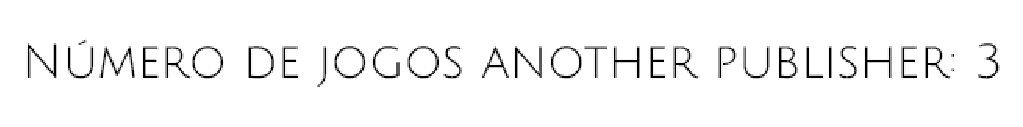
\includegraphics[scale=0.5]{figuras/another_publisher.eps}
	\caption{Número de jogos publicados por outra empresa}
	\label{image:another}
	\end{figure}
	\item Gráfico que compara os números de jogos que foram publicados pela desenvolvedora pelo números de jogos que foram publicados por outra empresa por ano. A figura \ref{image:anotherxown} é uma representação da métrica.
	\begin{figure}
	\centering
	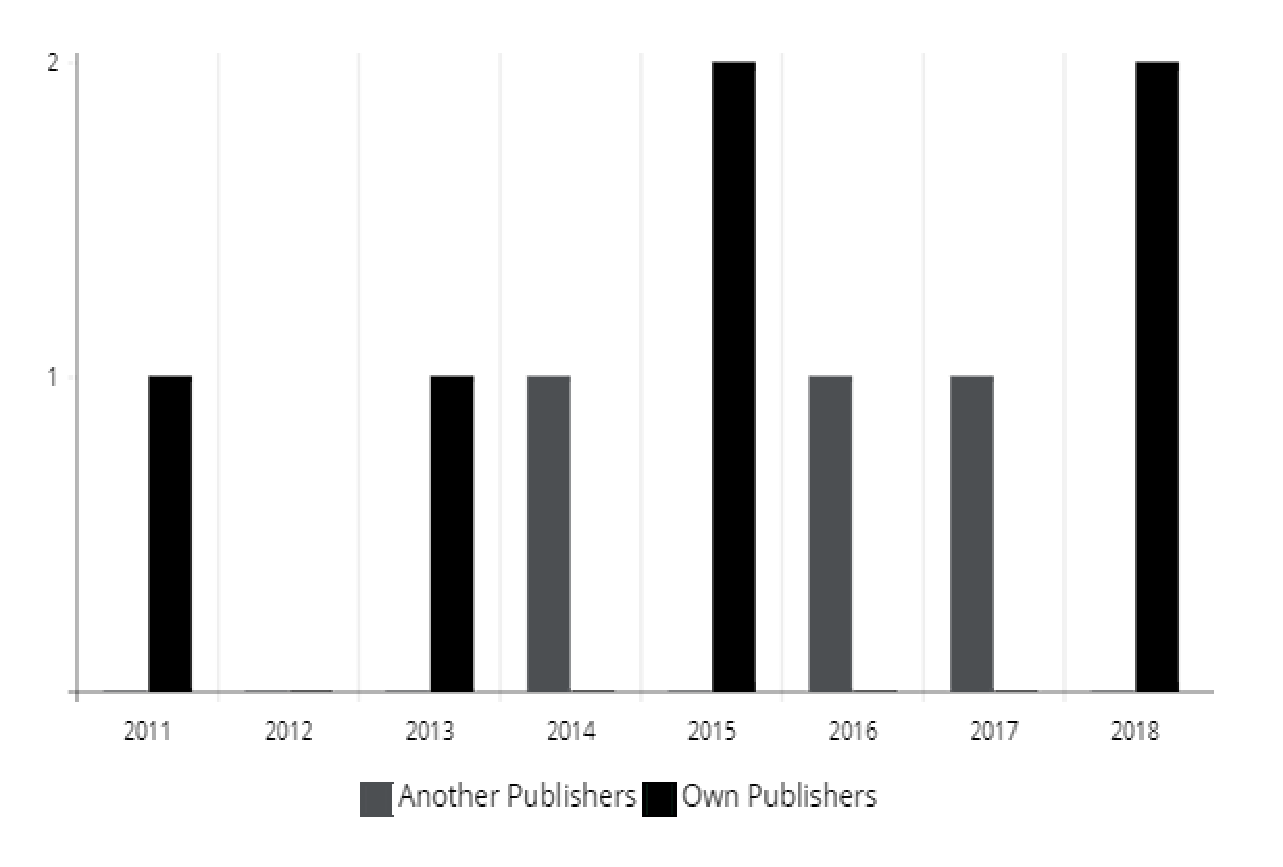
\includegraphics[scale=0.4]{figuras/anotherxown.eps}
	\caption{Outra Publicadora x Própria Desenvolvedora}
	\label{image:anotherxown}
	\end{figure}
	\item Tabela de quantos jogos daquele determinado perfil atingiram um número \textit{N} de donos e sua porcentagem. A representação desta tabela fica evidenciada pela tabela \ref{table:num_donos}.
	\item Tabela de quantos jogos daquele determinado perfil atingiram um número \textit{N} de avaliações positivas e sua porcentagem. A representação desta tabela fica evidenciada pela tabela \ref{table:avaliacao}
	\item Gráfico de desenvolvedoras por número de jogos desenvolvidos. A figura \ref{image:developers} é uma representação da métrica.
	\begin{figure}
	\centering
	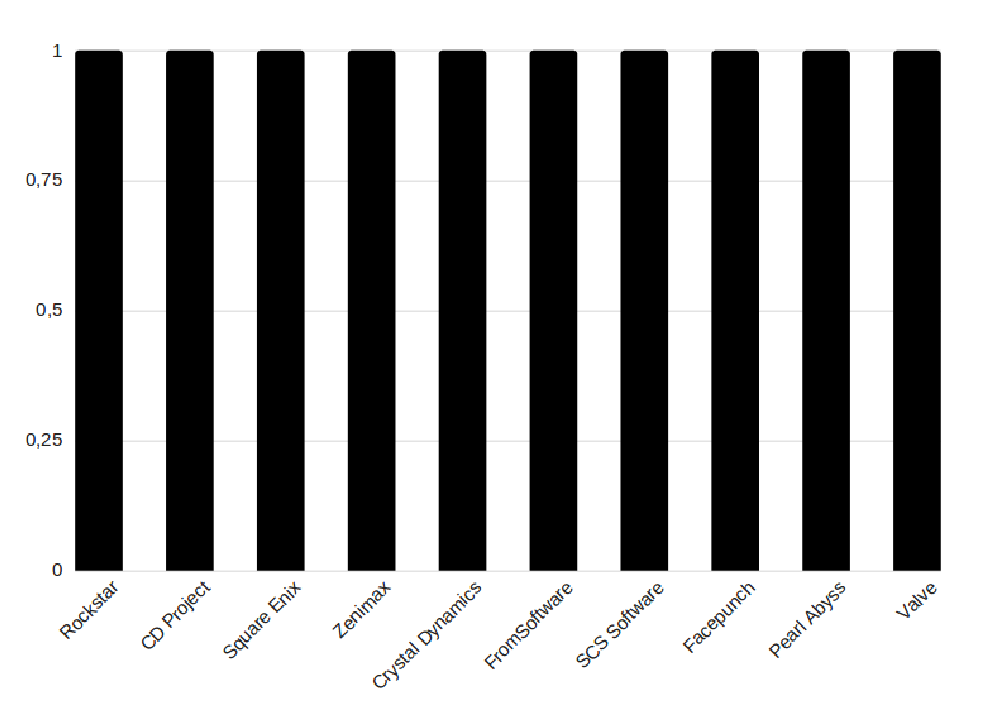
\includegraphics[scale=0.4]{figuras/developer.eps}
	\caption{Desenvolvedoras x Número de Jogos}
	\label{image:developers}
	\end{figure}
	\item Gráfico de linguangens suportados por número de jogos que a suportam. A figura \ref{image:languages} é uma representação da métrica.
	\begin{figure}
	\centering
	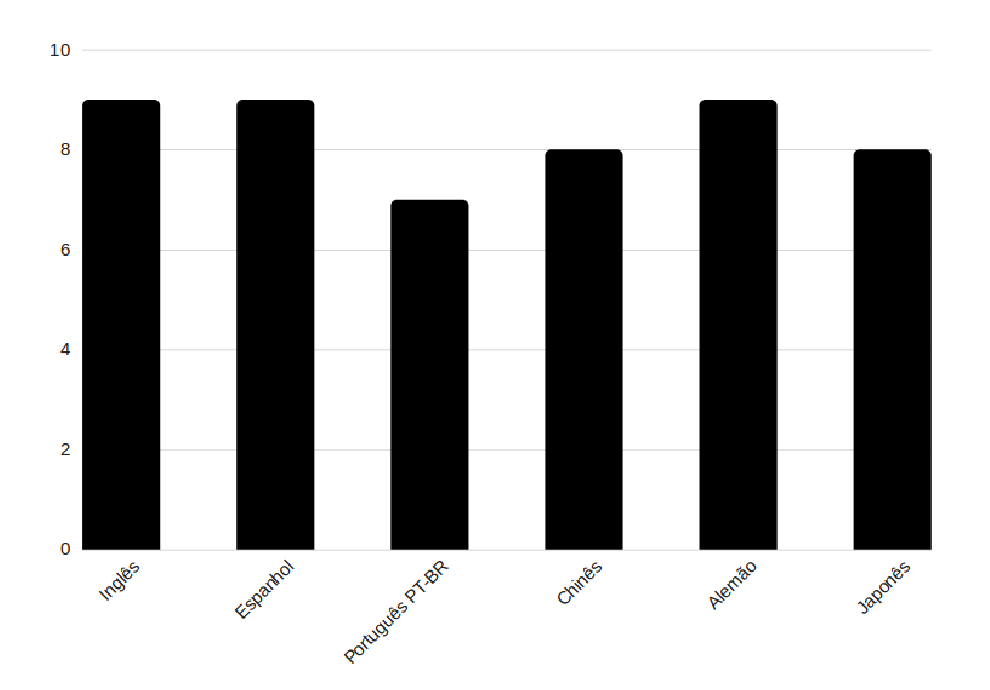
\includegraphics[scale=0.4]{figuras/language.eps}
	\caption{Linguagens Suportados x Número de Jogos}
	\label{image:languages}
	\end{figure}
\end{itemize}
\begin{table}
\centering
\begin{tabular}{|p{5cm}|p{5cm}|p{5cm}|}
\hline \textbf{Número de Donos} & \textbf{Quantidade de Jogos} & \textbf{\% de Jogos} \\
\hline 0 - 10000 & 10 & 100 \% \\
\hline 10000 - 50000 & 10 & 100 \% \\
\hline 50000 - 100000 & 9 & 90 \% \\
\hline 100000 - 500000 & 9 & 90 \% \\
\hline 500000 - 1000000 & 9 & 90 \% \\
\hline 1000000 - 5000000 & 8 & 80 \% \\
\hline 5000000 - 10000000 & 3 & 30 \% \\
\hline 10000000 - 50000000 & 1 & 10 \% \\
\hline
\end{tabular}
\caption{Número de donos e sua porcentagem}
\label{table:num_donos}
\end{table}
\begin{table}
\centering
\begin{tabular}{|p{5cm}|p{5cm}|p{5cm}|}
\hline \textbf{Porcentagem de Avaliação} & \textbf{Quantidade de Jogos} & \textbf{\% de Jogos} \\
\hline 0 \%- 10 \% & 10 & 100 \% \\
\hline 11 \%- 20 \% & 10 & 100 \% \\
\hline 21 \%- 30 \% & 10 & 100 \% \\
\hline 31 \%- 40 \% & 10 & 100 \% \\
\hline 41 \%- 50 \% & 10 & 100 \% \\
\hline 51 \%- 60 \% & 10 & 100 \% \\
\hline 61 \%- 70 \% & 10 & 100 \% \\
\hline 71 \%- 80 \% & 8 & 80 \% \\
\hline 81 \%- 90 \% & 6 & 60 \% \\
\hline 91 \%- 100 \% & 4 & 40 \% \\
\hline
\end{tabular}
\caption{Porcentagem de avaliação}
\label{table:avaliacao}
\end{table}